\begin{pastexam}[label={px:ntu-111-dsaa-14}]{臺大資工所 111 學年度 第 14 題}
（單選）

(5 points) Consider a red-black tree with $n$ internal nodes, where $n$ is even. At most how many
of them can be a black node with one red child?
\begin{enumerate}[label=(\Alph*)]
\item $\frac{n}{2}$
\item $n$
\item $\lfloor\log_2(n+1)\rfloor-1$
\item $\lfloor\log_2(n+1)\rfloor$
\item none of the other choices
\end{enumerate}
\end{pastexam}

\begin{pastsoln}
答案是 (A) $\frac{n}{2}$。

「black node with one red child」照字面讀成「恰好有一個紅色孩子的黑色節點」；讀成「至少一個」
答案也一樣，下面的上界兩種讀法都適用。 紅黑樹的性質照資結書第~10.3~節：根是黑的、紅色節點的孩子
都是黑的（外部節點 \textsc{nil} 算黑的）、從任一節點往下到每個 \textsc{nil} 經過的黑色節點數相同。

\textbf{上界 $n/2$。} 設這種黑色節點有 $k$ 個。 每一個都配上它的紅色孩子；不同的節點的孩子不會是
同一個（每個節點只有一個父節點），所以紅色節點至少 $k$ 個。 黑色、紅色合起來
$n \ge k + k$，$k \le n/2$。

\textbf{$n/2$ 做得到。} 定義一族樹 $T_b$：
\begin{itemize}
\item $T_1$：一個黑色節點，左孩子是紅色葉子。
\item $T_b$（$b \ge 2$）：黑色的根；左孩子是紅色節點，它的兩個子樹都是 $T_{b-1}$；右子樹是
$T_{b-1}$。
\end{itemize}
$T_b$ 的每條根到 \textsc{nil} 的路徑都恰好經過 $b$ 個黑色節點，紅色節點的孩子都是黑的，所以是
紅黑樹；而且\textbf{每一個}黑色節點都恰好有一個紅色孩子，紅、黑各佔一半。 節點數
$g(1) = 2$，$g(b) = 2 + 3g(b-1)$，得 $2, 8, 26, 80, \ldots$。 下圖是 $T_2$（$8$ 個節點，$4$ 個
符合條件的黑色節點；黑底白字是黑色節點，紅框是紅色節點）：
\begin{center}
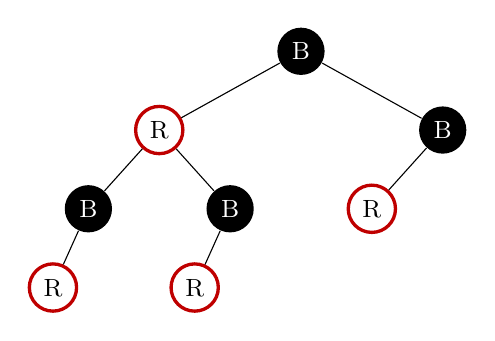
\begin{tikzpicture}[level distance=10mm,
  level 1/.style={sibling distance=36mm}, level 2/.style={sibling distance=18mm},
  level 3/.style={sibling distance=9mm},
  bk/.style={circle,fill=black,text=white,minimum size=6mm,inner sep=0pt,font=\small},
  rd/.style={circle,draw=red!75!black,very thick,minimum size=6mm,inner sep=0pt,font=\small}]
\node[bk] {B}
  child {node[rd] {R}
    child {node[bk] {B} child {node[rd] {R}} child[missing]}
    child {node[bk] {B} child {node[rd] {R}} child[missing]}}
  child {node[bk] {B} child {node[rd] {R}} child[missing]};
\end{tikzpicture}
\end{center}
$T_3$ 正好有 $26$ 個節點、$13$ 個符合條件的黑色節點，也就是下一題（歷屆試題~\ref{px:ntu-111-dsaa-15}）
說的「達到上一題答案的 $26$ 個節點的紅黑樹」。

\textbf{逐項檢查。}
\begin{itemize}
\item (A) 對：$n/2$ 是上界，而且有樹做得到（例如 $n = 26$）。
\item (B) $n$：比上界 $n/2$ 大，不可能（紅色節點自己就不算）。
\item (C)、(D)：$n = 26$ 時是 $3$ 和 $4$，但 $T_3$ 有 $13$ 個，所以它們不是「最多」。
\item (E)：(A) 成立，不選。
\end{itemize}
補充：$n/2$ 只有在 $n = 2, 8, 26, 80, \ldots$ 這些大小才達得到（下一題證明達到時樹一定長成 $T_b$）；
其他偶數，例如 $n = 4$，最多只有 $1$ 個。 選項問的是最緊的上界，答 (A)。
\end{pastsoln}
